\clearpage
\section{Comparing Between ASR Expansion and DEF Expansion Simulation Result}

%*******10********20********30********40********50********60********70********80

Here the 2 expansion simulation results are compared to analysis the similarities and difference between ASR and DEF expansion.

For ASR, 100x100x100mm model with 30\%  aggregate is chosen, of which 75\% of total aggregates are ASR reactive.

For DEF, same 100x100x100mm model with 30\%  aggregate is using, of which the 75x75x75mm at the center part is given intensified DEF expansion, and decreased gradually in the surrounding part.

\begin{figure}[!h]
\centering
\begin{subfigure}{.5\textwidth}
  \centering
  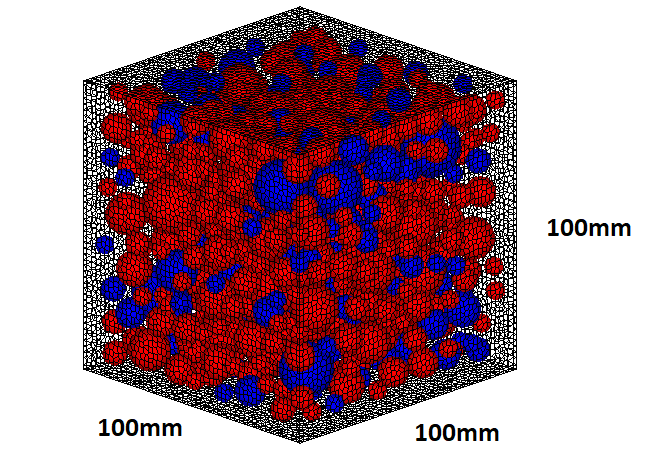
\includegraphics[width=.8\linewidth]{Files/Aggregate/A30P75.png}
  \caption{Model for ASR Expansion}
  \label{fig:A15_model}
\end{subfigure}%
\begin{subfigure}{.5\textwidth}
  \centering
  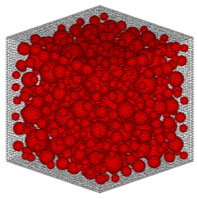
\includegraphics[width=.6\linewidth]{Files/Aggregate/A30.png}
  \caption{30\% Coarse Aggregate}
  \label{fig:A15_model}
\end{subfigure}
\caption{Model for DEF Expansion}
\label{fig:Aggregate_Percentage}
\end{figure}

\clearpage

\begin{figure}[ht]
\centering

    %*******
    \begin{subfigure}{.5\textwidth}
      \centering
      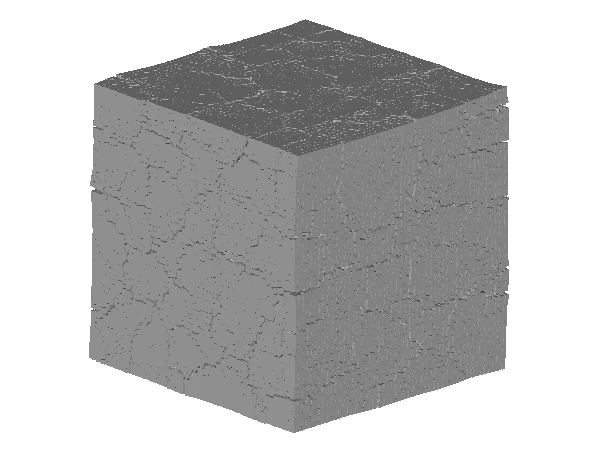
\includegraphics[width=.8\linewidth]{Files/exp_3D/ASR/A30P75_3_3d.png}
      \caption{75\% ASR Reactive Aggregate, \\3D Surface Cracks, 0.4223\% Expansion}
    \end{subfigure}%
    \begin{subfigure}{.5\textwidth}
      \centering
      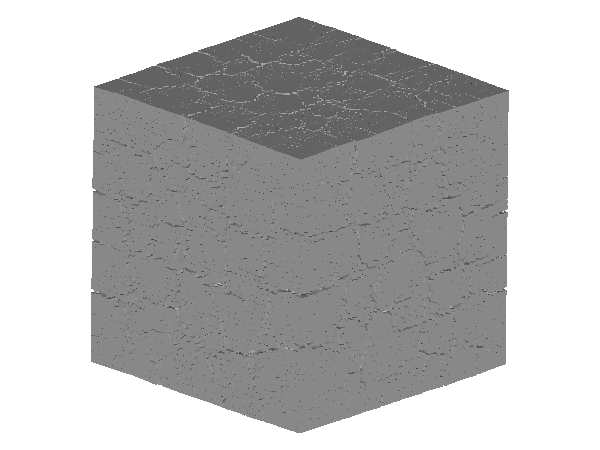
\includegraphics[width=.8\linewidth]{Files/exp_3D/DEF/A30X-5C_3_3d.png}
      \caption{75x75x75mm Intensified, \\ 3D Surface Cracks, 0.5118\% Expansion}
    \end{subfigure}
    %*******
    \begin{subfigure}{.5\textwidth}
      \centering
      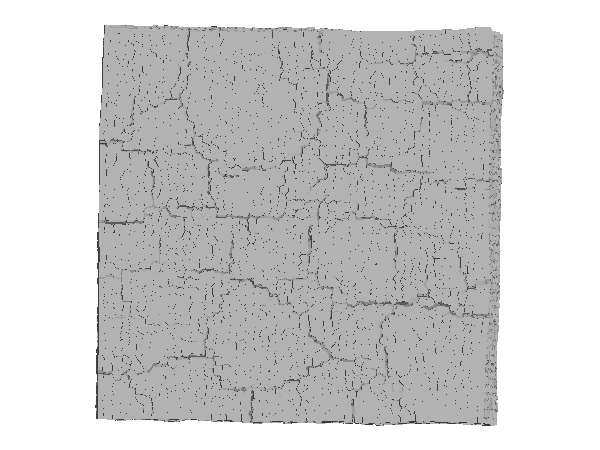
\includegraphics[width=.8\linewidth]{Files/exp_3D/ASR/A30P75_3_3ds.png}
      \caption{75\% ASR Reactive Aggregate, \\Surface Sideview, 0.4223\% Expansion}
      \end{subfigure}%
      %*******
    \begin{subfigure}{.5\textwidth}
      \centering
      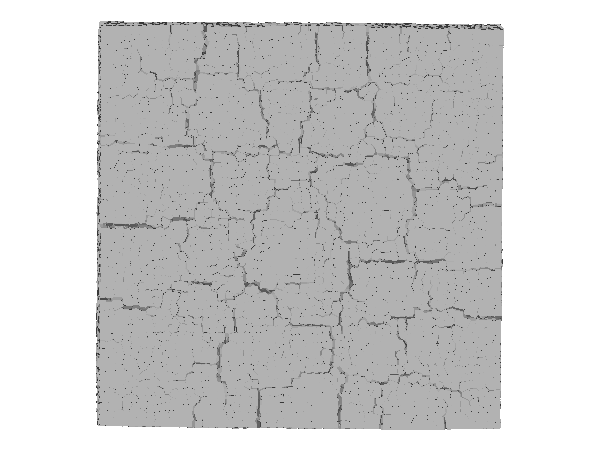
\includegraphics[width=.8\linewidth]{Files/exp_3D/DEF/A30X-5C_3_3ds.png}
      \caption{75x75x75mm Intensified DEF, \\ Surface Sideview, 0.5118\% Expansion}
      \end{subfigure}
      %*******
      %*******
      \begin{subfigure}{.5\textwidth}
        \centering
        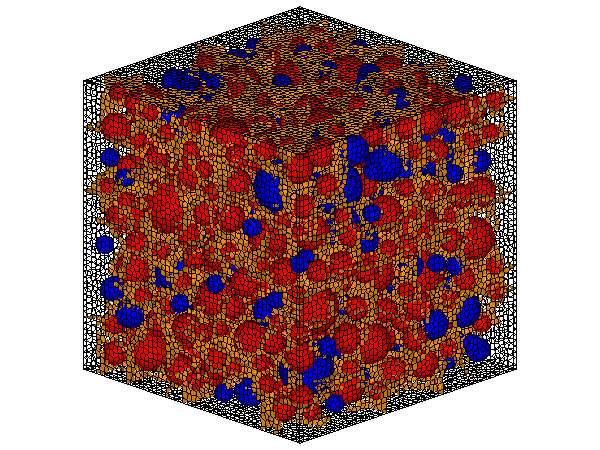
\includegraphics[width=.8\linewidth]{Files/exp_3D/ASR/A30P75_3_c.png}
        \caption{75\% ASR Reactive Aggregate, \\Inner Crack, 0.4223\% Expansion}
        \end{subfigure}%
        %*******
      \begin{subfigure}{.5\textwidth}
        \centering
        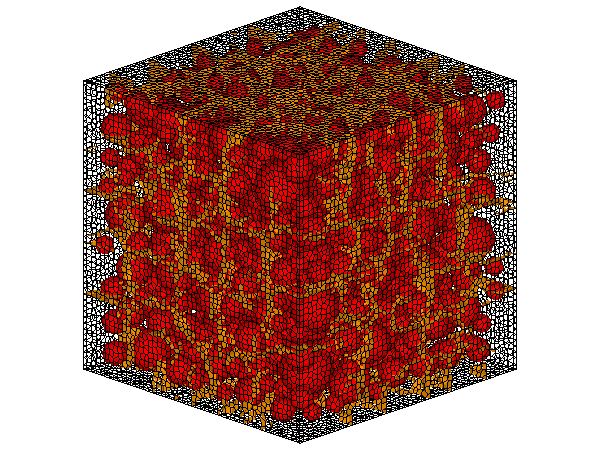
\includegraphics[width=.8\linewidth]{Files/exp_3D/DEF/A30X-5C_3_c.png}
        \caption{75x75x75mm Intensified DEF, \\Inner Crack, 0.5118\% Expansion}
        \end{subfigure}
        %*******
  \caption{Cracks Compare Between ASR Expansion and DEF Expansion Simulation Result}
  \label{fig:ASRvsDEF_3D}
\end{figure}

From Figure \label{fig:ASRvsDEF_3D} it can be seen that at a relatively close global expansion ratio, the surface cracking pattern of ASR expansion and DEF expansion can be very close.

However, the inner crack distribute is not exactly the same in these 2 cases. Clear cross alike distribution can be seen in DEF expanded case but not in ASR case.

This can also be confirmed by the cross-section view (Figure \ref{fig:ASRvsDEF_IS}), where in middle of each face of DEF expanded model concentration of crack perpendicular to surface is shown. Besides, for the DEF expansion, the inner part of the model is more integrated comparing to ASR case, with almost no crack inside.

This may indicate with similar outside cracking damage level, deteration caused by DEF expansion is less severe compared with ASR expansion.

\begin{figure}[ht]
\centering

    %*******
    \begin{subfigure}{.5\textwidth}
      \centering
      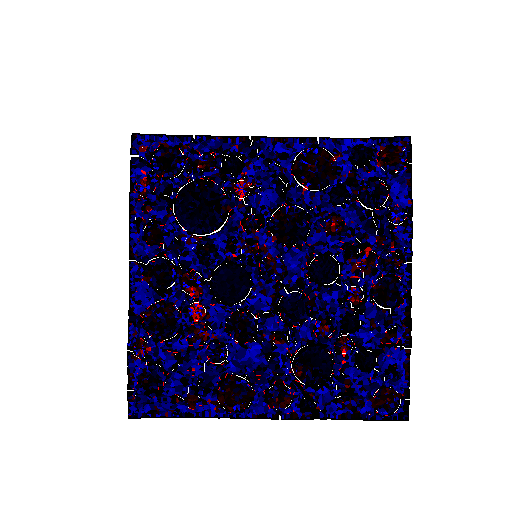
\includegraphics[width=.8\linewidth]{Files/exp_3D/ASR/A30P75_3_stress.png}
      \caption{75\% ASR Reactive Aggregate, \\ Cross Section, 0.4223\% Expansion}
    \end{subfigure}%
    %*******
    \begin{subfigure}{.5\textwidth}
      \centering
      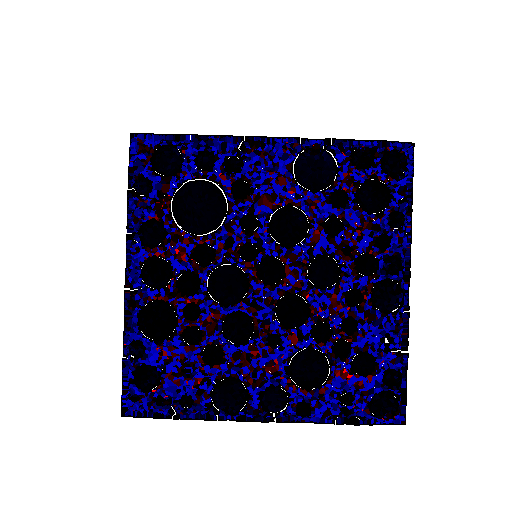
\includegraphics[width=.8\linewidth]{Files/exp_3D/DEF/A30X-5C_3_stress.png}
      \caption{75x75x75mm Intensified DEF, \\ Cross Section, 0.5118\% Expansion}
    \end{subfigure}

    \begin{subfigure}{0.8\textwidth}
  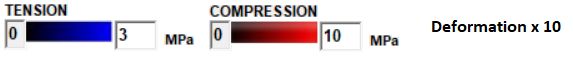
\includegraphics[width=0.8\linewidth]{Files/exp_3D/tagCS10.png}
\end{subfigure}%


  \caption{Cross Section Compare Between ASR Expansion and DEF Expansion Simulation Result (Deformation x 10)}
  \label{fig:ASRvsDEF_IS}
\end{figure}

\begin{table}[!h]
\centering
\begin{tabular}{ |p{4cm}|p{5cm}|p{5cm}| }
\hline
 Crack Width [mm] &  ASR A30P75 0.4223\% Expansion Total Cracked Interfaces  &  DEF A30I75 0.5118\% Expansion Total Cracked Interfaces \\
 \hline\hline

   0.00000 - 0.00005 & 316744 & 373019 \\
   0.00005 - 0.00010 & 286704 & 335814\\
   0.00010 - 0.00020 & 263943 & 299690\\
   0.00020 - 0.00050 & 234672 & 249242\\
   0.00050 - 0.00100 & 183238 & 177030\\
   0.00100 - 0.00300 & 131553 & 113350\\
   0.00300 - 0.01000 & 42432 & 42207\\
   0.01000 - 0.03000 & 275 & 240\\
   0.03000 - 0.10000 & 0 & 0\\
   0.1000+ & 0 & 0\\

  \hline
  \end{tabular}
\caption{Expansion in Each Step for A30 P75 Case 3}
\label{table:A30P75_3_Cracks}
\end{table}

%TODO:plot

PLOT

When comparing the cracked interfaced grouped by the width of crack (Tabel \ref{table:A30P75_3_Cracks}), it also can be seen that comparing to ASR expansion, cracks in DEF expansion simulation result is more concentrated in smaller crack width,  which is under 0.001mm in this comparison.


ASR and DEF expansion, though similar on their surface cracking, are different in their mechanism and inner condition. And the simulation used in this research can properly reproduce not only the similarities but also the difference between them.
